\documentclass[a4paper,12pt]{article}
\usepackage[margin=1in]{geometry} % Adjust margins if needed
\usepackage{amsmath} % Paquete para escribir matemáticas
\usepackage{ulem} % Importar el paquete ulem
\usepackage{graphicx}
\usepackage{float}
\usepackage{parskip}
\usepackage{caption}
\usepackage{subcaption}
\usepackage{caption}
\usepackage{siunitx}
\usepackage{graphicx}
\usepackage{circuitikz,siunitx}
\usepackage{tikz}

\captionsetup[figure]{name=Fig.} % Change the label for figures

\title{TP4 - Teoría de Circuitos 1\\ Acoplamiento Magnético y Cuadripolos}

\author{Autores: \\Pla, Juan Ignacio (63486)\\Torino, Joaquín (63140)\\Caviglia, Facundo (63178)\\Belsito, Ramiro (62641)}
\date{Actualizado: \today}

\begin{document}
\maketitle

\section{Introducción}
\hspace{1cm} El objetivo de este experimento es trasladar los conocimientos teóricos sobre 
el acoplamiento magnético y sobre los cuadripolos a la práctica. Por restricciones de tiempo,
la sección del estudio de cuadripolos no se pudo realizar.

\hspace{1cm}Para desarrollar el experimento, se utilizarán bobinas que nos permitan intercambiar
el núcleo, de forma tal que los mismos bobinados cambiarán su comportamiento según la 
permitividad magnética del aluminio, del hierro y del hierro laminado. Se analizará la reacción
del transformador ante una carga en el circuito secundario, mediante la medición de las caídas de
tensión en la misma y el cálculo previo de las inductancias propias y mutuas con el núcleo correspondiente.


\section{Materiales utilizados}

\begin{itemize}
\item Fuente de tensión alterna regulable, configurada en \textit{Vef} = 30v y a \textit{f} = 50Hz.
\item Dos bobinados con núcleo abierto y resistencias internas de 21,5$\Omega$ y \\
23$\Omega$
respectivamente.
\begin{figure}[H]
    \centering
    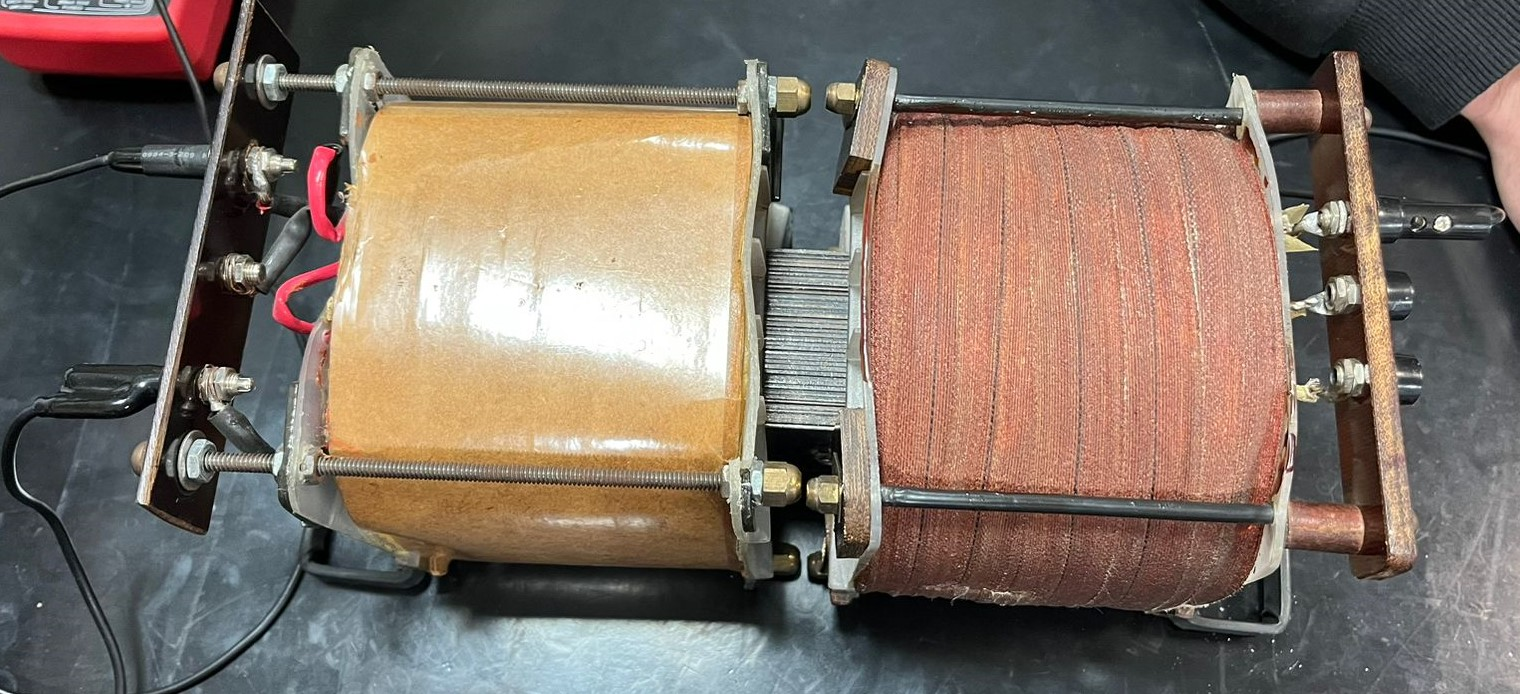
\includegraphics[width=0.5\linewidth]{bobinados.jpg}
    \caption{Bobinados}
\end{figure}

\item Núcleo de hierro sólido, de hierro laminado y de aluminio.
\item Multímetros digitales en los modos de: Óhmetro, Voltímetro y Amperímetro.
\item Resistencia de 200$\Omega$.
\end{itemize}
\section{Desarrollo}

\subsection{Homología}
\hspace{1cm} Antes de analizar el circuito, se debe determinar la homología de las inductancias. Para ello, se llevará
a cabo una conexión del primer bobinado a la fuente de tensión variable, de \textit{f} = 50Hz, con el segundo bobinado
acoplado magnéticamente mediante el núcleo compartido por ambos.

\begin{figure}[H]
    \centering
    \begin{circuitikz}[american, cute inductors, scale=0.5]
        \draw (0,0) to[sV,invert,l=$30v$ $50Hz$] (0,3)
                    to[R, l=$21.5\Omega$] (4,3)
                    to[L, l_=$L_1$] (4,0)
                    to[short] (0,0);
        \draw [fill=black] (3.5,2)node(a){} circle (2pt) ++(3.2,0)node(b){} circle (2pt);
        \draw [<->,>=stealth] (3.5, 3.5)  to [bend left] node[above](c) {M} ++(3.1,0);
        \draw (6,3) to[short] (8,3);
        \draw (6,3) to[L, l=$L_2$] (6,0)
                    to[short] (8,0);
        \draw [fill=black] (8,3) node(d){} circle (2pt);
        \draw [fill=black] (8,0) node(e){} circle (2pt);
        \draw [<->,>=stealth] (4.55, 2.5)  to [] node[above, font=\footnotesize](c) {$v_1$} ++(1,0);
        \draw [<->,>=stealth] (4.55, 2.2)  to [] node[below, font=\footnotesize](c) {$v_2$} (5.5,0.7);
    \end{circuitikz}
    \caption{Circuito 1}
\end{figure}

\hspace{1cm} A continuación, se determinará la homología midiendo la tensión entre uno de los bornes del primer inductor y 
cada uno de los bornes del segundo. Es decir, se debe comparar la tensión $v_1$ y $v_2$ presentes en la "Fig.2:Circuito 1".
Concluyendo que el par homólogo se encuentra en aquel borne cuya tensión es menor. Esto se debe a que al medir la tension entre 
bornes homologos, se esta midiendo la tension entre los dos extremos positivos de ambas bobinas. Cuando se mide la tensión 
entre un borne positivo y otro negativo, la diferencia de tension será mayor que la anterior ya que la diferencia incluira la 
caída de potencial en la bobina que se cambia de polaridad.

\hspace{1cm} Mediante mediciones experimentales, pudimos identificar las grandes diferencias que existen en utilizar distintos
núcleos para acoplar magnéticamente los bobinados. Los resultados podrán verse en las tablas en las siguientes secciones. Pero,
teóricamente hablando, esto se debe a que hay núcleos, como el hierro, con mayor permitividad magnética $\mu$.


\subsection{Cálculo de Inductancias}

\hspace{1cm} Para obtener los valores de inductancia propia, se realizó un ensayo con el circuito secundario abierto y el primario
conectado a la fuente de tensión variable. Se midió la caída de tensión en los bornes del primario con el voltímetro y la corriente
que circulaba por el mismo con un amperímetro.

\hspace{1cm} De esta forma, considerando que la corriente en el circuito secundario es nula, dado que este se encuentra abierto,
se conocen los valores de resistencia ($R=21.5 \Omega$), tensión ($30v$) y corriente del circuito primario ($i_1$ - como se puede apreciar
en la "Fig.3:Circuito 2" -). Aplicando la ecuación de mallas correspondiente, se puede obtener el valor de la inductancia propia del 
primario, siendo este el único valor desconocido de la ecuación.

\begin{equation}
    (V_1) = (R_1\cdot i_1 + jwL_1\cdot i_1)
    \Longleftrightarrow
    |\frac {V_1}{i_1}| = \sqrt{(R_1)^2 + (wL_1)^2 }
\end{equation}

\begin{figure}[H]
    \centering
    \begin{circuitikz}[american, cute inductors, scale=0.5]
        \draw [->] (0.3,3) -- (0.4,3) node[midway,above] {$i_1$};
        \draw (0,0) to[sV,invert,l=$30v$ $50Hz$] (0,3)
                    to[R, l=$21.5\Omega$] (4,3)
                    to[L, l_=$L_1$] (4,0);
        \draw (0,0) to[short] (1,0)
                    to[ammeter] (3,0)
                    to[short] (4,0);
        \draw [fill=black] (3.5,2)node(a){} circle (2pt) ++(3.2,0)node(b){} circle (2pt);
        \draw [<->,>=stealth] (3.5, 3.5)  to [bend left] node[above](c) {M} ++(3.1,0);
        \draw (6,3) to[short] (8,3);
        \draw (6,3) to[L, l=$L_2$] (6,0)
                    to[short] (8,0);
        \draw [fill=black] (8,3) node(d){} circle (2pt) ++(0,-3)node(e){} circle (2pt);
        \draw [<->,>=stealth] (8, 2.8)  to [] node[right, font=\footnotesize](c) {$v_2$} ++(0,-2.6);
    \end{circuitikz}
    \caption{Circuito 2}
\end{figure}

\hspace{1cm} Para calcular el valor de la inductancia propia del segundo bobinado, se realizó el mismo ensayo pero con la fuente
de tensión variable conectado a este y el circuito primario abierto. Luego se hizo uso de la ley de mallas con los valores
obtenidos para el circuito secundario.

\begin{equation}
    (V_2) = (R_2\cdot i_2 + jwL_2\cdot i_2)
    \Longleftrightarrow
    |\frac {V_2}{i_2}| = \sqrt{(R_2)^2 + (wL_2)^2 }
\end{equation}

\begin{figure}[H]
    \centering
    \begin{circuitikz}[american, cute inductors, scale=0.5]
        \draw [->] (0.3,3) -- (0.4,3) node[midway,above] {$i_2$};
        \draw (0,0) to[sV,invert,l=$30v$ $50Hz$] (0,3)
                    to[R, l=$23\Omega$] (4,3)
                    to[L, l_=$L_2$] (4,0);
        \draw (0,0) to[short] (1,0)
                    to[ammeter] (3,0)
                    to[short] (4,0);
        \draw [fill=black] (3.5,2)node(a){} circle (2pt) ++(3.2,0)node(b){} circle (2pt);
        \draw [<->,>=stealth] (3.5, 3.5)  to [bend left] node[above](c) {M} ++(3.1,0);
        \draw (6,3) to[short] (8,3);
        \draw (6,3) to[L, l=$L_1$] (6,0)
                    to[short] (8,0);
        \draw [fill=black] (8,3) node(d){} circle (2pt);
        \draw [fill=black] (8,0) node(e){} circle (2pt);
    \end{circuitikz}
    \caption{Circuito 3}
\end{figure}

\hspace{1cm} En el caso de la inductancia mutua, se utilizó el mismo ensayo que nos permitió determinar la inductancia propia del primer
bobinado ("Fig.3:Circuito2") y se obtuvo el valor de la caída de tensión en los bornes del bobinado secundario abierto ($v_2$). Por ende,
considerando que dicha caída corresponde a:
\begin{equation}
    |V_2| = |-j\cdot w\cdot L_2\cdot i_1\cdot M|
    \Longleftrightarrow
    M = |\frac{V_2}{w\cdot L_2\cdot i_1}|
\end{equation}
\begin{equation}
    K = \frac{M}{\sqrt{L_1\cdot L_2}}
\end{equation}

\subsection{Resultados Obtenidos}
\hspace{1cm} En esta tabla se pueden observar todos los datos obtenidos en el experimento, tanto los valores medidos como 
los calculados.
\begin{figure}[h!]
    \centering
    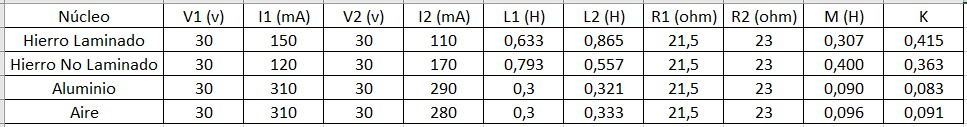
\includegraphics[width=\linewidth]{tabla1.jpg}
    \caption{Resultados obtenidos}
    \end{figure}

    \section{Conexión de Resistencia en el Secundario}
\hspace{1cm} En el siguiente experimento, se conectó una resistencia de $R_d$ = 200$\Omega$ en el circuito secundario y se midió 
la caída de tensión determinada como $V_2$. Se hizo un análisis de la caída de potencial $V_2$ y tambíen de la corriente que circula
por el circuito secundario, para cada uno de los núcleos utilizados.

\begin{figure}[H]
    \centering
    \begin{circuitikz}[american, cute inductors, scale=0.5]
        \draw (0,0) to[sV,invert,l=$30v$ $50Hz$] (0,3)
                    to[R, l=$21.5\Omega$] (4,3)
                    to[L, l_=$L_1$] (4,0)
                    to[short] (0,0);
        \draw [fill=black] (3.5,2)node(a){} circle (2pt) ++(3.2,0)node(b){} circle (2pt);
        \draw [<->,>=stealth] (3.5, 3.5)  to [bend left] node[above](c) {M} ++(3.1,0);
        \draw (6,3) to[short] (10,3)
                    to[R, l=$R_d$] (10,0);
        \draw (10,3) to[short] (14,3)
                    to[voltmeter, l=$v_2$] (14,0)
                    to[short] (10,0);
        \draw (6,3) to[L, l=$L_2$] (6,0);
        \draw (6,0) to[short] (7,0)
                    to[ammeter] (8.5,0)
                    to[short] (10,0);
        \draw [->] (6.3,3) -- (8.4,3) node[midway,above right] {$i_2$};

    \end{circuitikz}
    \caption{Circuito 4}
\end{figure}

\subsection{Mediciones Experimentales}

\begin{figure}[h]
    \centering
    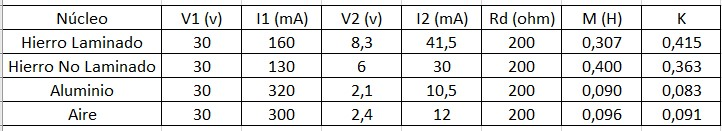
\includegraphics[width=\linewidth]{tabla2.jpg}
    \caption{Resultados obtenidos con $R_d$ conectado en el circuito secundario}
    \end{figure}

\subsection{Analisis de Errores}
\hspace{1cm} Dada la naturaleza experimental de las mediciones realizadas, los errores son inevitables y es de vital importancia reconocerlos.
Primero y principal, la posición de los núcleos dentro de las bobinas fue determinada de manera completamente experimental. Se trato de que la 
ubicación sea lo más imparcial posible, pero no se efectuó ninguna medición rigurosa para asegurarse de que esto sea asi. Sin embargo, esta 
particularidad queda reflejada en el valor de $K$, por lo cual no es algo que este obviado en los resultados. Finalmente, errores como la 
resistencia de los cables, variaciones en la fuente de tensión, fluctuaciones en el  autotransformador y hasta las limitaciones físicas del 
multímetro digital son todos factores que reducen en cierta medida la calidad de las mediciones. Sin embargo, a pesar de estas fuentes de error, 
los efectos estudiados pudieron seguir siendo apreciados y no se modificó la calidad de la experiencia, que no tenía como objetivo la toma de 
valores perfectos sino la apreciación de fenómenos electromagnéticos entre dos bobinados.

\subsection{Análisis de Resultados y Conclusión}
\hspace{1cm} Puede notarse en las tablas anteriores, que cada resultado depende enormemente del núcleo utilizado. Esto se debe a que 
dependiendo de las propiedades del mismo, las bobinas compartirán mayor o menor flujo de campo magnético, lo cual afecta tanto a las 
inductancias propias como a la inductancia mutua y por ende el coeficiente de acoplamiento, como puede verse en los resultados obtenidos
por la Fig.5. Por ejemplo, el núcleo de hierro laminado ayuda a disminuir pérdidas por corrientes de Foucault.
\\En la Fig.7 se puede observar que la caída de tensión y la corriente en el circuito secundario son mayores cuando se utilizan 
los núcleos de hierro, mientras que las menores se obtienen con el núcleo de aluminio, que posee una baja permeabilidad magnética.
Entendiendo la correlación directa entre las tensiones $v_2$ encontradas en el secundario y la energía que el bobinado primario
transfiere a través del acoplamiento magnético.

\end{document}